\documentclass{article}
\usepackage[utf8]{inputenc}
\usepackage[spanish]{babel}
\usepackage{listings}
\usepackage{graphicx}
\graphicspath{ {images/} }
\usepackage{cite}

\begin{document}

\begin{titlepage}
    \begin{center}
        \vspace*{1cm}
            
        \Huge
        \textbf{Informa2 S.A.S}
            
        \vspace{0.5cm}
        \LARGE
        Parcial 2 - Análisis y diseño 
            
        \vspace{1.5cm}
            
        \textbf{Carolina Jimenez Restrepo}\\
          \textbf{c.c 1020470694}
            
        \vfill
            
        \vspace{0.8cm}
            
        \Large
        Despartamento de Ingeniería Electrónica y Telecomunicaciones\\
        Universidad de Antioquia\\
        Medellín\\
        Septiembre de 2021
            
    \end{center}
\end{titlepage}

\tableofcontents
\newpage
\section{Sección introductoria}\label{intro}
En el presente informe se mostrara el análisis y diseño realizado para dar solucion al parcial 2 de la materia informatica, en el se mostraran los pasos y tareas propuestas para lograr cumplir el objetivo.

\subsection{Análisis y diseño}
\
Luego de leer y analizar el desafío propuesto para el parcial 2 se tiene una idea de cómo dar solución a este, lo primero que se debe tener en cuenta son los requerimientos del desafío, el cual nos pide ajustar las dimensiones de una imagen para proyectarlas en una matriz de LEDs RGB, así mismo como crear la matriz y hacer el montaje de la parte eléctrica que permitirá su funcionamiento.\\

Para la parte de ajustar las dimensiones de la imagen que sería submuestreo (disminución de la resolución) y sobremuestreo (aumento de la resolución) se creara un código que realice estos procesos, sin ayuda de librerías como lo indican las instrucciones del desafío, el siguiente paso es guardar una nueva imagen con estas nuevas dimensiones para luego obtener los datos correspondientes a los colores que componen la imagen y escribirlos en un archivo txt del cual se copiara la informacion y se  utilizará en la plataforma tinkercad para la generación de una matriz de colores que junto con otras líneas de código nos permitirán ver la imagen proyectada en la matriz de LEDs RGB.\\

Para el montaje de la matriz LEDs RGB se utilizan 14 tiras de LEDs RGB lo cual nos genera una matriz 14x14 un Arduino y una fuente de voltaje que nos permitirán alimentar la matriz.\\
Para el desarrollo del algoritmo se crea en el entorno Qt una clase que va a permitir realizar el proceso de escalado de imagen (submuestreo y sobremuestreo), guardar la nueva imagen y comprobar si lo cargado es una imagen y otra clase que permitira obtener los valores de los colores RGB que conforman la imagen a proyectar, que seran cargados en una matriz y luego guardados en un txt. Las clase y métodos mencionados pueden variar a medida que se va desarrollando el proyecto.

\subsection{Esquema}
\
Las tareas definidas para el desarrollo del algoritmo son:\\
Montaje de la matriz LEDs RGB: En tinkercad se utilizan 14 tiras de NeoPixels así se crea una matriz LEDs de 14x14, esta matriz se complementa con un Arduino y una fuente de alimentación de 5v la cual debe ir conectada a al pin de voltaje del Arduino 5V, los cuales permitirán el funcionamiento de la matriz.\\

Lectura y verificación de la imagen: El algoritmo recibe la dirección donde se encuentra ubicada una imagen, luego de esto verifica si lo que se encuentra en dicha ubicación si es una imagen o corresponde a otro tipo de archivo, si lo verificado es diferente a una imagen mostrara un mensaje de error, en caso contrario, si es una imagen procede a realizar el escalado de la imagen.\\

Proceso de escalado de imagen: Se aplica el código desarrollado para el submuestreo o sobremuestreo de la imagen, el cual genera una nueva imagen con las nuevas dimensiones que se adapta a la matriz LEDs RGB que ya tenemos creada en tinkercad, el proceso de escalado combina redimencionar la imagen con un proceso de ir pasando pixel por pixel y mezclar cada color RGB que la compone para asi lograr un buen escalado. Este proceso se aplica en procesamiento de imagenes, para tener este conocimiento fue necesario consultar varias fuentes sobre procesamiento de imagenes, digitalización de imagenes,conocer como utilizaban los colores RGB y algunos cogidos utilizados para su desarrollo.\\

Obtención de valores: Luego de aplicar el código de escalado de imagen se obtienen los valores equivalentes a los colores que contiene la imagen, estos valores se muestran en una matriz la cual se guarda en un archivo txt y luego se copian en el código implementado en tinkercad.\\

La proyección de la imagen: En tinkercad al tener la matriz que contiene los colores y el código que permite el funcionamiento de la matriz de LEDs se toman los valores que se encuentran en la matriz, se recorre y esos mismos valores se representan en la matriz de LEDs (proyección de la imagen).

\subsection{Algoritmo}

1.	Tener una imagen guardada que se quiera proyectar en la matriz LEDs.\\
2.	Se ingresa la ubicación de la imagen\\
3.	Lectura de la imagen.\\
4.	verificación de imagen, si la imagen es correcta (es una imagen) va al siguiente paso si es incorrecta muestra mensaje de error y debe volver a ingresar la ubicación.\\
5.	comprobar si la imagen a proyectar necesita sobremuestreo o submuestreo, si es sobremuestreo se aumenta la resolución, si es submuestreo se disminuye la resolución.\\
6.	ejecutar el proceso de escalamiento (escogido en el punto anterior).\\
7.	Genera una nueva imagen con el escalamiento.\\
8.	Obtención de valores de los colores RGB que componen la imagen.\\
9.	Crear matriz con los colores obtenidos.\\
10.	Crear un archivo txt.\\
11.	Escribir la matriz que contiene la información de los colores en un archivo .txt.\\
12.	Abrir el archivo .txt con un editor de texto.\\
13.	Copiar la información que contiene el archivo txt.\\
14.	Pegar e ingresar en la parte de código de tinkercad donde se tiene la matriz LED.\\
15.	Ejecutar el código que se encuentra en tinkercad.\\
16.	Proyectar la imagen en la matriz de LEDs RGB.\\

\subsection{Consideraciones}

Lo planteado en el análisis y deseño esta sujeto a cambios ya que en el transcurso de la implementación de la solución planteada pueden surgir nuevas ideas o problemas que necesiten una solución diferente a lo planteado.\\
Los esquemas y diagramas están desarrollados de una manera global pero tratando de ser lo más claro posibles para la comprensión del proceso que se desea realizar.\\
La matriz de LEDs debe ser de un tamaño par para que la proyeccion de la imagen se vea mejor.\\
Las tareas se realizaran en el orden establecido para así tener un buen  avance, disminuir los imprevistos y cumplir con el objetivo en el tiempo establecido.

\section{Inclusión de imágenes} \label{imagenes}
\subsection{Matriz LEDs}
En la Figura (\ref{fig:Matriz leds.png}), se presenta la matriz de LEDs con la que se trabajara, esta matriz esta dispuesta a cambios segun lo requiera el avance del desafio.

\begin{figure}[h]
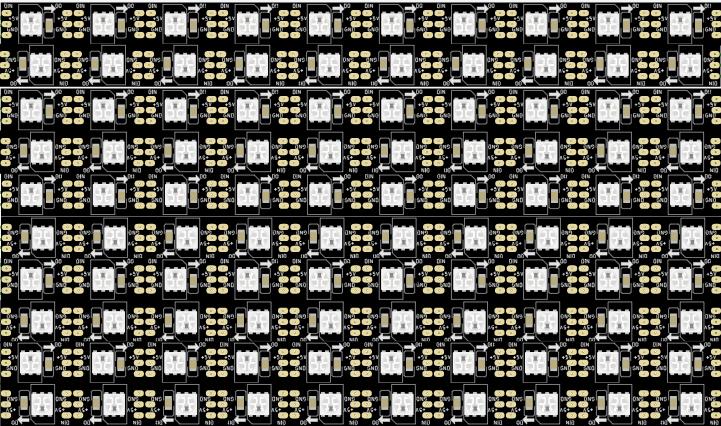
\includegraphics[width=9cm]{Matriz leds.png}
\centering
\caption{Matriz LEDs RGB}
\label{fig:Matriz leds.png}
\end{figure}

\subsection{Esquema}
En la Figura (\ref{fig:Tareas a realizarpng}), se presenta el esquema de las tareas a realizar repartidas por bloques los cuales indican las tareas que se desean lograr juntas.

\begin{figure}[h]
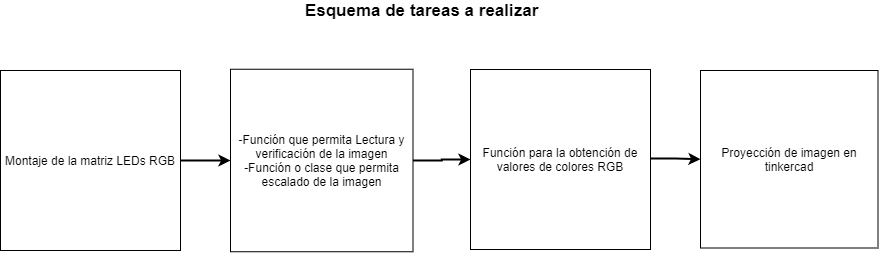
\includegraphics[width=8cm]{Tareas a realizar.png}
\centering
\caption{Esquema tareas}
\label{fig:Tareas a realizarpng}
\end{figure}

\subsection{Diagra de flujo}
En la Figura (\ref{fig:Diagramaparcial.png}), se presenta el diagrama de flujo del algoritmo planteado.

\begin{figure}[h]
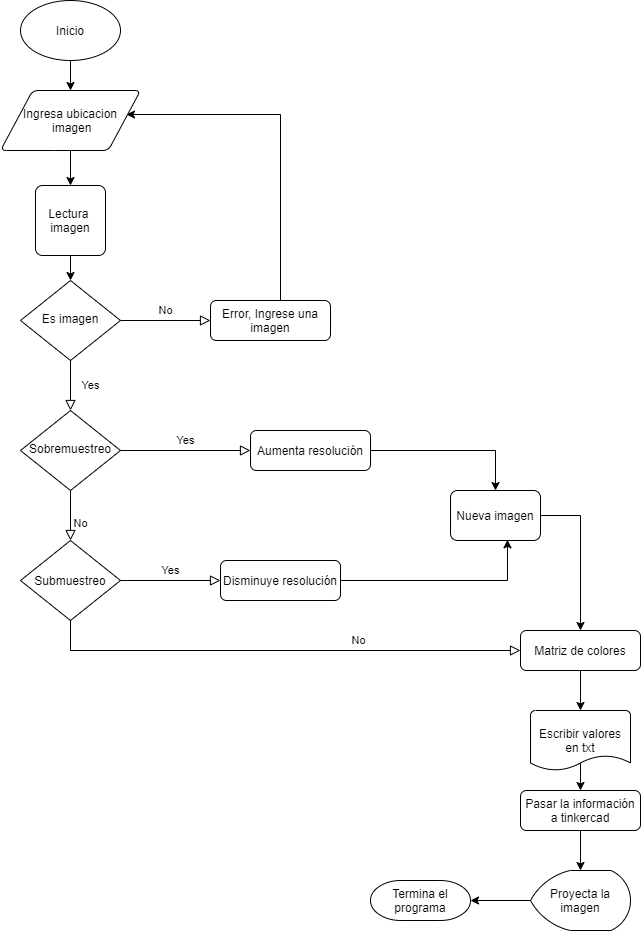
\includegraphics[width=7cm]{Diagramaparcial.png}
\centering
\caption{Diagrama de flujo}
\label{fig:Diagramaparcial.png}
\end{figure}

\bibliographystyle{IEEEtran}
\cite{Digitalizacionwebsite}.\\\\
\bibliography{references}

\end{document}
